\scanpage{4}
\deleted{\unsure{Rappel|Rapp.}}

\uline{Graphes}

\[
\begin{aligned}
\text{\uline{Def}}\\[-2pt]\text{\uline{Graphe}}
\end{aligned}
\quad
\left\{\begin{aligned}
&\text{Ens } S\ \text{de ``sommet''}\\
&\text{ens } A\ \text{``d'arêtes''}\\
&R\subset S\times A\qquad\text{relation d'incidence}
\end{aligned}\right\}
\ \text{Données}
\]

\uline{\unsure{Axiome|Axiomes}} \quad 1) $\forall a\in A,\ \unsure{\exists|\exists s}\ \operatorname{card}R\{a\}=2$ (tte arête a exactement 2 sommet)

\noindent\begin{minipage}[t]{.32\linewidth}
\figure{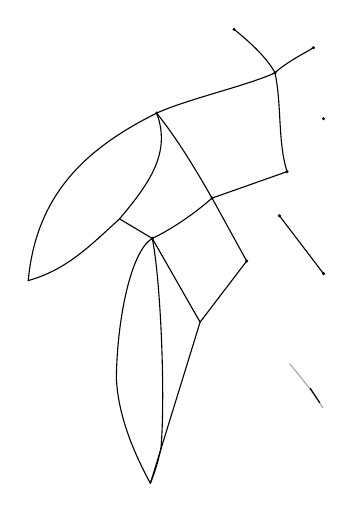
\begin{tikzpicture}[x=.008cm,y=-.008cm,line cap=round,line join=round]
\draw (492,496) .. controls (511,511) and (544,540) .. (557,565)
  .. controls (575,548) and (604,534) .. (618,525);
\draw (557,565) .. controls (514,585) and (417,607) .. (369,629)
  .. controls (263,682) and (178,753) .. (165,895);
\draw (165,895) .. controls (226,878) and (263,840) .. (310,797)
  .. controls (359,739) and (392,691) .. (369,629);
\draw (369,629) .. controls (404,673) and (431,719) .. (457,764)
  -- (576,722) .. controls (561,672) and (568,619) .. (557,565);
\draw (310,797) -- (362,828) .. controls (394,813) and (431,787) .. (457,764)
  -- (512,864) -- (438,961) -- (362,828);
\draw (362,828) .. controls (328,848) and (306,957) .. (305,1050)
  .. controls (308,1116) and (338,1178) .. (359,1217);
\draw (362,828) .. controls (375,891) and (383,1071) .. (376,1160)
  .. controls (371,1185) and (365,1202) .. (359,1217);
\draw (438,961) -- (359,1217);
\draw (564,792) -- (634,884);
% Detached smudged pen stroke; not asserted to be an edge of the graph.
\draw[opacity=.35] (580,1027) .. controls (603,1054) and (618,1074) .. (633,1097);
\draw (613,1066) -- (628,1089);
\foreach \x/\y in {492/496,618/525,557/565,369/629,576/722,457/764,362/828,512/864,564/792,634/884,634/638}
  \fill (\x,\y) circle[radius=2.7];
\end{tikzpicture}}
\end{minipage}\hfill
\begin{minipage}[t]{.63\linewidth}
Un graphe est dit \deleted{\unsure{quelq|qqch|quelq.}} \uline{strict} si une arête est connue quand on connait ses sommets.

\deleted{\unsure{Un|On}} La donnée d'un \uline{graphe strict} équivaut donc \unsure{à 2|à la} donnée d'un ens. $S$, et d'une partie $A$ de $\unsure{\mathfrak{P}|\mathcal{P}}_{2}(S)$ (ens des parties de card. 2 de $S$).
\end{minipage}

Arc d'un graphe (ou arête orientée) -- ens $\vec A$

\deleted{\uline{\unsure{Remarque}}} Réalisation topologique d'un graphe
\[
\deleted{X(S,A,R)=\bigl(S\amalg(\vec A\times I)\bigr)/.}
\]

a) Segment associé à un ens $a$ de card. 2
\[
\begin{aligned}
\bigl[\,\deleted{\unsure{\operatorname{réal}|\operatorname{rel}}}\inserted{\operatorname{seg}}(a)&\subset I^{a}\qquad (I=[0,1])\\
\operatorname{seg}(a)&=\bigl\{\{t_{\unsure{x|n}}\}_{x\in a}\mid\textstyle\sum t_x=1\bigr\}\ ;\ \text{on a }\ a\hookrightarrow\operatorname{seg}(a)
\end{aligned}
\]

b)
\[
\operatorname{réal}(S,A,R)=\left(S\amalg\coprod_{a\in A}\operatorname{seg} R\{a\}\right)\big/\begin{aligned}&\text{\unsure{relation}}\\&\text{d'équiv.}\end{aligned}
\]

\deleted{Réalisation} \quad [ \unsure{Si|On} a $X=\coprod_{a\in A}\operatorname{seg}R\{a\}$, on a
\diagram{\begin{tikzcd}[ampersand replacement=\&,row sep=0.2em,column sep=1.7em]
\partial X \arrow[r] \& S\\[-2pt]
\cap \& {}\\[-2pt]
X \& {}
\end{tikzcd}}
et on ``\unsure{attache}'' $X$ \unsure{:|à} $S$ \unsure{par|$\vdash$} $\partial X\to S$ \quad ]

``Réalisation \inserted{\unsure{géom}} rectiligne'' d'un graphe (fini..) dans un vectoriel (de dim finie\ldots) sur $\mathbb{R}$ : homéom. dans
% archive sheet number: 3
